% Source: graduate-coursework/Sp26/CSCE775/course_notes/bellman_equation_guide.tex
% Description: Future rewards shrink. A \$5 tip one hour from now is only worth \$4.50 in ``today dollars.''

\documentclass[border=4pt]{standalone}
\usepackage{amsfonts}
\usepackage{amsmath}
\usepackage{amssymb}
\usepackage{amsthm}
\usepackage[T1]{fontenc}
\usepackage{graphicx}
\usepackage{tikz}
\usepackage{xcolor}
\usetikzlibrary{arrows.meta, positioning, shapes.geometric, calc, decorations.pathreplacing}

\definecolor{Garnet}{HTML}{73000a}
\definecolor{SecondaryBlue}{HTML}{466A9F}
\definecolor{SecondaryGreen}{HTML}{65780B}
\definecolor{FlatRed}{HTML}{CC2E40}
\definecolor{FlatDark}{HTML}{1F414D}
\definecolor{FlatYellow}{HTML}{CED318}
\definecolor{FlatGold}{HTML}{A49137}
\definecolor{LightGray}{HTML}{F0F0F0}

\renewcommand{\baselinestretch}{1.2}
\newcommand{\vocab}[1]{\textbf{\textcolor{Garnet}{#1}}}
\newcommand{\mathhighlight}[1]{\textcolor{SecondaryBlue}{#1}}

\begin{document}
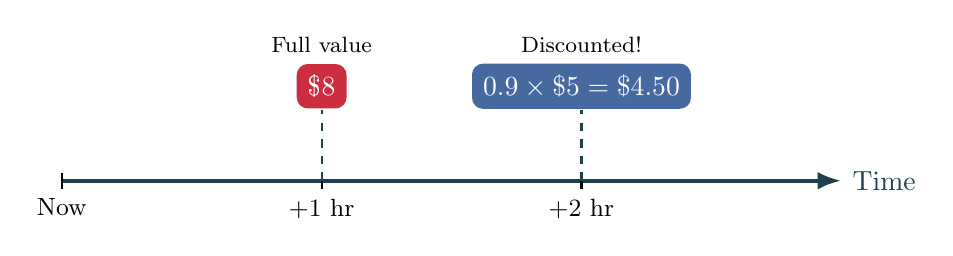
\begin{tikzpicture}[x=2.2cm, y=1cm, thick]
        % Timeline Line
        \draw[->, -{Latex[length=3mm]}, FlatDark, line width=1.5pt] (0,0) -- (4.5,0) node[right] {Time};

        % Ticks
        \foreach \x/\t in {0/Now, 1.5/+1 hr, 3/+2 hr} {
            \draw (\x,0.1) -- (\x,-0.1) node[below] {\small \t};
        }

        % Rewards with actual values
        \node[fill=FlatRed, text=white, inner sep=4pt, rounded corners] at (1.5, 1.2) {\$8};
        \node[fill=SecondaryBlue, text=white, inner sep=4pt, rounded corners] at (3, 1.2) {$0.9 \times \$5 = \$4.50$};

        \draw[dashed, FlatDark] (1.5, 0) -- (1.5, 0.9);
        \draw[dashed, FlatDark] (3, 0) -- (3, 0.9);

        % Labels
        \node[above, font=\footnotesize] at (1.5, 1.5) {Full value};
        \node[above, font=\footnotesize] at (3, 1.5) {Discounted!};

    \end{tikzpicture}
\end{document}
